\chapter{Introduction}
\label{ch:introduction}
66 Million years ago, an asteroid the size of Rotterdam initiated what is perhaps the most well known cataclysmic event in the history of life on Earth. With an impact releasing the energy of a billion nuclear bombs, the asteroid left a 180 km crater in the Gulf of Mexico. Launching enough debris into the atmosphere to block out the light of the Sun, eventually leading to the extinction of three quarters of spiecies on Earth, most famously the non-avian dinosaurs (\cite{DinosaurAsteroid}). In recorded human history, a multitude of noteworthy asteroids have impacted Earth, such as the Tunguska impactor in 1908 in Siberia. Flattening over 2000 km$^2$ of forest, events such as this serve as a staunch reminder of the massive kinetic energy that can be released by an object descending to Earth from space, and the danger this poses to human civilization.\\

Cognizant of such hazard, the United States launched the Spaceguard Survey in 1992, aiming to ``identify 90\% of near-Earth Asteroids (NEA's) larger than 1 km within 10 years.'' (\cite{Spaceguard}). With improvements in observation technology, more meteors were witnessed and recorded, leading to greater awareness into the frequency and unpredictability of such events. Of course, impacts from space are not a problem exclusive to Earth; as the 1994 impact of comet Shoemaker-Levy 9 into Jupiter proved. This impact showed that impacts of objects large enough to cause global catastrophy were not as highly improbably as once considered, and asteroid identification efforts took off with it.\\

The initial spaceguard survey goal was completed succesfully, and it is known that there are - within reasonable probability - no civilization-ending asteroids destined for Earth impact in the coming millenium. Nevertheless, smaller asteroids can still pose a local threat to human life or property. In addition, much is still unknown about the exact population of near-Earth asteroids, and such knowledge might provide valuable insights into the origin and evolution of the Solar system. Therefore, NASA extended the spaceguard mandate to detect 90\% of all NEA's larger than 140m (\cite{SpaceguardHistory}). \\

Since then, a lot of progress has been made in cataloguing and identifying smaller NEA's. Additionally, consideration has been given to survey for smaller limiting diameters (e.g. \cite{2003NEOSDT}). However, such efforts have to date still been very unsuccesful: For example, in 2013, a meteoric airburst over the city of Chelyabinsk, Russia, seriously injured almost 1500 people and damaged several thousands of buildings. Although damage was limited due to the high altitude of the explosion, no precautionary measures were taken, as the asteroid was completely unknown until the moment of atmospheric entry. Luckily, such events are not a common occurence. However, the large majority of NEA's of this size is completely unknown, and as such they can strike anywhere at any time. 

\section{Near-Earth Asteroids}
\label{sec:introduction_NEA}
Asteroids are perhaps the most diverse object in the Solar system: ranging in size from tiny chips to dwarf planets such as Vesta and Ceres; from rocky compositions, to fully metallic monoliths, and composites in various elements and mineral shapes; from close to the Sun on short orbits, to distant eccentric long period trajectories. All of this greatly increases the complexity of surveying for near-Earth asteroid. Before continuing, the definition of a near-Earth asteroid will be given as follows: \textit{a near-Earth asteroid is any asteroid with a perihelion $q \leq 1.3 \mathrm{AU}$ and semi-major axis $a \leq 4.2 \mathrm{AU}$}. \\

Current knowledge of the asteroid population is based on past and current NEA surveys. The most important parameter to consider is the size-frequency distribution of the objects. After all, larger objects exhibit a larger impact energy and hence threat, but small objects are more common and harder to detect. A good representation for this size-frequency distribution is a power law as follows:
\begin{equation}
 \frac{dN}{dD_p} \propto D_p^{-k}
 \label{eq:sizefreqlaw}
\end{equation}
With exponent $k$ in the range of 2.95 - 3.5 (\cite{AsteroidSizeFrequency}). Commonly, the size of the asteroid can not be directly ascertained; the target is too small to accurately determine the size. However, estimates can be made based on the absolute magnitude $H$ of the object by relation with an assumed albedo $p_v$ ($p_v = 0.14$ is often used as an approximation) using the relationship first derived by \cite{AsteroidSizeAlbedo}:
\begin{equation}
 D = \frac{1329 \mathrm{km}}{\sqrt{p_v}}\cdot 10^{-H/5}
 \label{eq:asteroidsize}
\end{equation}
As a result of the success of the spaceguard survey efforts, past efforts have more than likely identified all NEA's with $H \leq 15$, corresponsing to the \textit{flying mountains} several kilometers in diameter. Also, at smaller limiting diameters, a lot of NEA's have been - and continue to be - found. The surveys through which this is achieved will be discussed in further detail in \autoref{sec:insec:introductionidentification}. Through a process of modelling the asteroid population, and simulating the performance of past surveys on it, followed by fitting the results, \cite{GranvikPopulation} have produced a parametric model of the NEA population. The distribution of orbital elements in this model can be seen in \autoref{fig:population_histogram}. \\

\begin{figure}[htbp]
 \centering
 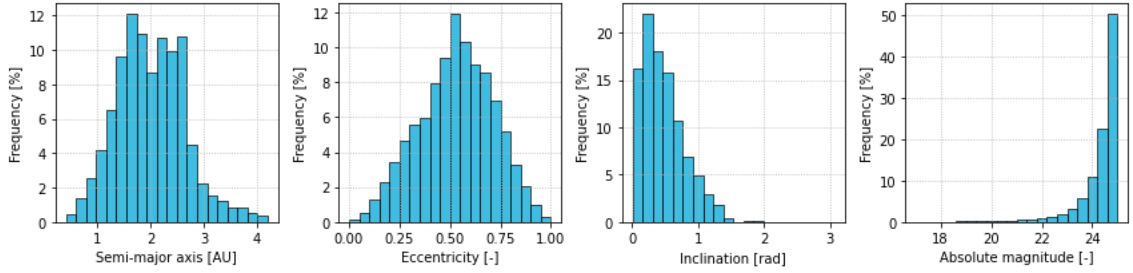
\includegraphics[width=1.0\textwidth]{img/population_histogram.png}
 \caption{Frequency of orbital elements for modelled NEA population according to \cite{GranvikPopulation}}.
 \label{fig:population_histogram}
\end{figure}

Several things are of note: First and foremost, the population is very diverse; there is no particular concentration of NEA's anywhere that allows for simple exploitation in survey design. Secondly, the bulk of NEA's has a semi-major axis of $1.0 \mathrm{AU} < a < 3.0 \mathrm{AU}$. The dips at $a = 2.0 \mathrm{AU}$ and $a = 2.5 \mathrm{AU}$ correspond to the 4:1 and 3:1 orbital resonance with Jupiter, respectively. The inclination of asteroids is concetrated among the ecliptic, but very low inclinations are rare due to gravitational interactions with the planets. Lastly, the effect of \autoref{eq:sizefreqlaw} can be seen: 50\% of the asteroids in the population generated by \cite{GranvikPopulation} has $24.6 \leq H < 25$, corresponding to a diameter of $D \leq 40 \mathrm{m}$. \\

Among these small NEA's was the asteroid which entered Earth's atmosphere over Chelyabinsk in 2013. It is currently estimated that this asteroid had a diameter of 17 to 20 meters (\cite{ChelyabinskNASA}). Assuming an albedo of $p_v = 0.14$, this would give it an absolute magnitude of $H \approx 26.5$. As previously discussed, completeness at these limiting diameters is very low. \autoref{fig:completeness_size} shows the completeness as a function of size according to \cite{HarrisPopulation}. They estimate that, at their time of writing, less than 0.005\% of all asteroids of this size have been identified. Through new and continued survey efforts, \cite{2017NEOSDT} project that the completeness at this size will increase to approximately 1.5\% by 2023. \\

\begin{figure}[htbp]
 \centering
 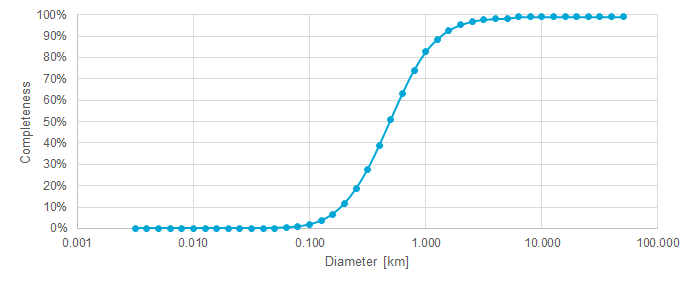
\includegraphics[width=0.75\textwidth]{img/completeness_size.png}
 \caption{Expected survey completeness as a function of near-Earth asteroid diameter. \cite{HarrisPopulation}}
 \label{fig:completeness_size}
\end{figure}

The problem can be seen in more detail in \autoref{fig:population_estimates}. Here, \cite{HarrisPopulation} show the expected and identified population of NEA's as a function of their size. The effect of the continued spaceguard efforts can be seen clearly here: the asteroid population with $D > 1 \mathrm{km}$ is completely known, and the population of asteroids $D > 140 \mathrm{m}$ is nearing the targeted 90\% completion. However, as the search efforts have been designed specifically to identify targets at this limiting size, the population with $D < 100 \mathrm{m}$ is still by far and large undiscovered.

\begin{figure}[htbp]
 \centering
 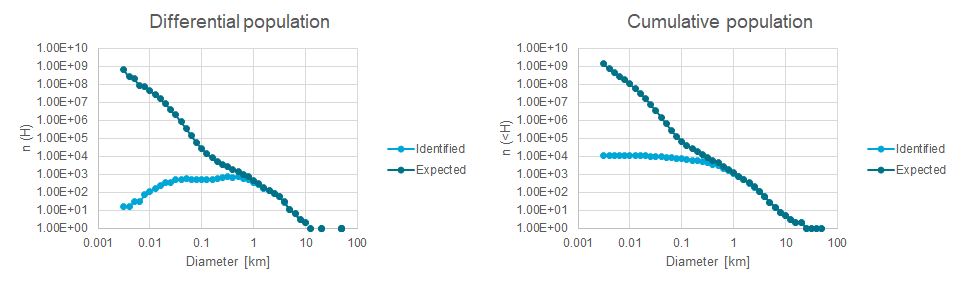
\includegraphics[width=1.0\textwidth]{img/population_estimates.png}
 \caption{State of asteroid identification progress as of August 2014, compared to the expected number of asteroids per diameter. Note that the y-axis is logarithmic. \cite{HarrisPopulation}}
 \label{fig:population_estimates}
\end{figure}


\section{Past and Current Identification Efforts}
\label{sec:introductionidentification}

Before continuing to the topic of the presented research, first some discourse shall be given to the missions that have resulted in the current knowledge of the NEA population. For brevity, not all missions will be listed; just a representative sample judged by the author to give a good overview of the state of the art. The missions are separated into two categories: space-based, and Earth-based. The latter comprises telescopes on Earth, with the advantage of having access to Earth infrastructure, supporting larger telescope apertures and providing practically unlimited electrical power, communication bandwidth, storage and computational resources. However, Earth-based systems are hindered by atmospheric distortion, extinction of light as it passes through the air, weather, limited search area depending on geographic position, and day-night cycles. Space-based systems contrast this: they are limited mostly by the maximum aperture of the telescopes they can support, the on-board processing capabilities and the computational power. Atmospheric and weather effects are mostly non-existant in space, however interference from the Sun, Earth and Moon should not be underestimated. To date, all NEA surveys from space have been carried out from orbits around Earth. Some proposals for deep space missions will be discussed in \autoref{sec:introductionproposals}.\\

In \autoref{fig:identification_per_survey}, the contribution of several surveys to the total catalogue of NEAs is shown. The two largest contributors, the Catalina Sky Survey and the Pan-STARRS observatories, were both constructed to accomplish the goal of bringing the NEA survey completeness for asteroids $D > 140 \mathrm{m}$ to over 90\% of the population. The effect of these purpose-built observatories can be easily seen in their volume of discoveries. Through improvement to the facilities and processing pipelines - e.g. through better computing resources - it can be seen that the number of discoveries is still undergoing a healthy amount of growth. It is therefore important to consider the impact these surveys have on the research and proposed missions.

\begin{figure}[htbp]
 \centering
 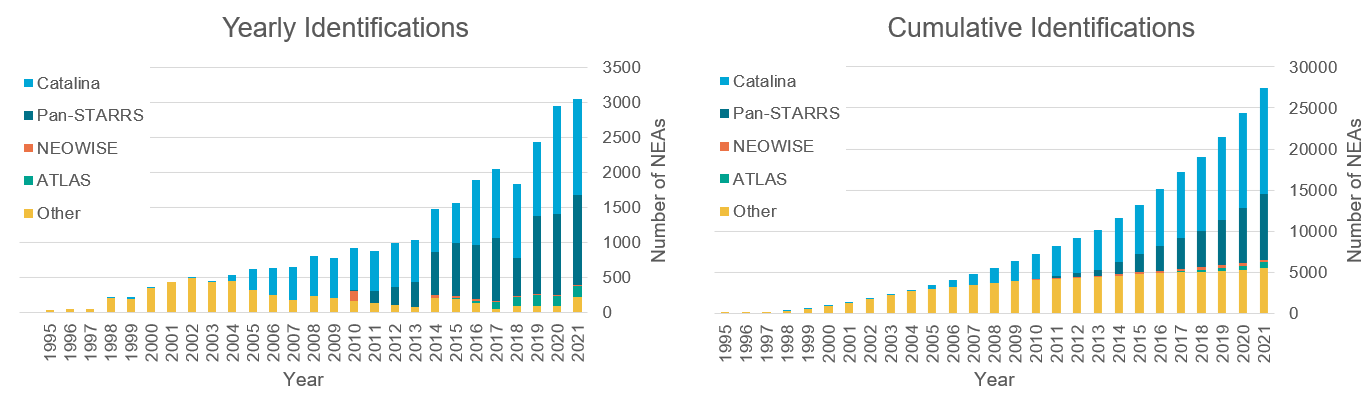
\includegraphics[width=1.0\textwidth]{img/identification_per_survey.png}
 \caption{Yearly and cumulative identifications made per NEA survey from 1995 up to and including 2021. Data obtained from \url{https://cneos.jpl.nasa.gov/stats}}
 \label{fig:identification_per_survey}
\end{figure}


\subsection{Earth-based Surveys}
With almost 13000 discoveries as of the end of 2021, the Catalina Sky Survey (CSS) is currently the most succesful NEA survey by volume of detections. Operated by the University of Arizona, the CSS operates a trio of telescopes in the Santa Catalina mountains: the primary telescope is a 1.5 meter wide field reflector telescope supported by a 1.0m follow-up telescope and a further 0.7m telescope, both catadioptric. The main telescope showcases the advantages of Earth-based surveys well, as it utilizes a 111 megapixel camera with a field of view of 5 square degrees. This allows it to image the sky at a very high frequency, down to a limiting magnitude of 21.5 (\cite{CatalinaSkySurvey}).\\

The second of the major NEA surveys is the Pan-STARRS project operated by the University of Hawaii. Operating two 1.8m catadioptric telescopes, equipped with 1.4 gigapixels camera sensors, it is capable of imaging down to a visual magnitude of 24. Currently, development is underway to expand Pan-STARRS to four telescopes, and allowing it to serve as a precursor for development of the software and data processing of the Large Synoptic Survey Telescope, which will be further discussed below (\cite{PANSTARRS}).\\

The last of the current large NEA surveys is the ATLAS (Asteroid Terrestrial-Impact Last Alert System) project. Contrary to the previously mentioned surveys, the goal of ATLAS is not to catalogue large quantities of NEAs, but to provide a last warning in case of incoming impactors. It is comprised of two 0.5m catadioptric telescopes, with plans to expand the system with three more sets of two telescopes. The survey is completely automated, and is tasked with providing impact warning for targets too small to impact until their last approach. The predicted warning times are between a day and a week (\cite{ATLAS}). Although this allows for alleviation of some of the damage, it is too short to take significant countermeasures such as an asteroid deflection mission or a large-scale evacuation. In addition, ATLAS suffers from the same problems as other Earth-based telescopes. For example, the 2013 Chelyabinsk meteor was not detected, as it approached Earth from the direction of the Sun.\\

Although not yet in operation, the expected impact of the Large Synoptic Survey Telescope (LSST) warrants a mention. Currently being constructed in the mountains of Chile, the LSST will utilize a three-mirror reflector with a 8.4m aperture, in combination with a 3.2 gigapixel sensor, making it the largest digital camera ever produced. It is expected to enter operations fully in October 2023, with a limiting magnitude of around 24.5 (\cite{LSST}). Although the LSST is expected to complete the goal of cataloguing 90\% of the $D > 140 \mathrm{m}$ NEA population in approximately 12 years, it can be seen from its limiting magnitude that detecting the faintest of NEAs will not be a succesful endeavor for an Earth-based survey, even at extreme apertures and sensor sizes. Therefore, a short overview of some space-based surveys will now be provided.\\

\subsection{Space-based Surveys}
As shown above, meaningfully increasing the survey completeness for asteroids under the $D > 140 \mathrm{m}$ threshold is best carried out by means of a survey from space. To date, no dedicated NEA survey spacecraft has been launched, however, several missions have discovered a significant number of NEAs, most prominently among those the NEOWISE mission. Initially used for the WISE mission, imaging the entire sky in near-infrared, the spacecraft was put into hibernation after the coolant for its camera sensor ran out. In 2013, it was reawakened for the NEOWISE mission, where it would use its sensors in a non-cryogenic mode to survey for NEAs. Although the number of NEAs detected by NEOWISE is small compared to the dedicated Earth-based surveys, the new objects detected by it have been small and dark: targets which are hard to impossible to image using visual telescopes from Earth (\cite{NEOWISEResult}). NEOWISE thereby has shown the capability of both a space-based survey and a survey using near-infrared sensors, and its findings have contributed greatly to the capabilities for modelling the NEA population (e.g. \cite{GranvikPopulation}).\\

Building on the success of NEOWISE, a new spacecraft is currently being developed by NASA under the NEOCam project. Aiming for a launch in 2026, the NEOCam mission has a dedicated design for identification of NEAs. Situated at the Sun-Earth L1 point, the mission will observe the space around Earth for potentially hazardous asteroids. It is expected that NEOCam is also capable of completing the 90\% survey completeness of asteroids $D > 140 \mathrm{m}$, and will be capable of imaging some asteroids down to $D > 30 \mathrm{m}$, although the latter is not a primary design goal (\cite{NEOCam}).

\section{Novel Proposals}
\label{sec:introductionproposals}
As an update to the new spaceguard objective, \cite{DefendingEarth} investigated the progress and goals of NEA cataloguing efforts. Their initial verdict was that current survey efforts are insufficient to meet the new goal, and new missions will be necessary. Several of these surveys have already been dicussed above. However, next to discussing NEAs with $D > 140 \mathrm{m}$, they also state that \textit{``... objects smaller than 140 meters in diameter are also capable of causing significant damage to Earth.''} and make the recommendation that \textit{``Because recent studies of meteor airbursts have suggested that near-earth objects as small as 30 to 50 meters in diameter could be highly destructive, surveys should attempt to detect as many 30- to 50-meter objects as possible.''}. \\

Leading among the current proposals is the work by NASA's Jet Propulsion Laboratory (\cite{2003NEOSDT}, \cite{2017NEOSDT}). The initial proposal centered around updating the limiting size of to-be-detected asteroids to lower limiting diameters. The authors investigate a multitude of possibilities for accomplishing the 90\% completeness at $D > 140 \mathrm{m}$ goal, as well as investigating the influence on smaller diameter asteroids. Their conclusion is in line with the aforementioned: the most promising option for cataloguing a multitude of NEA's is to perform a survey from deep space. Several options are considered, among which the best performing options are 0.5 meter aperture thermal infrared telescopes at Earth-Sun L1 or in Venus-trailing orbit. The authors note no significant gain in performance by sizing up the telescope. It is also noted that no full optimization for the orbit or payload is performed. However, the proposal shows a lot of potential. \\

\begin{figure}[htbp]
 \centering
 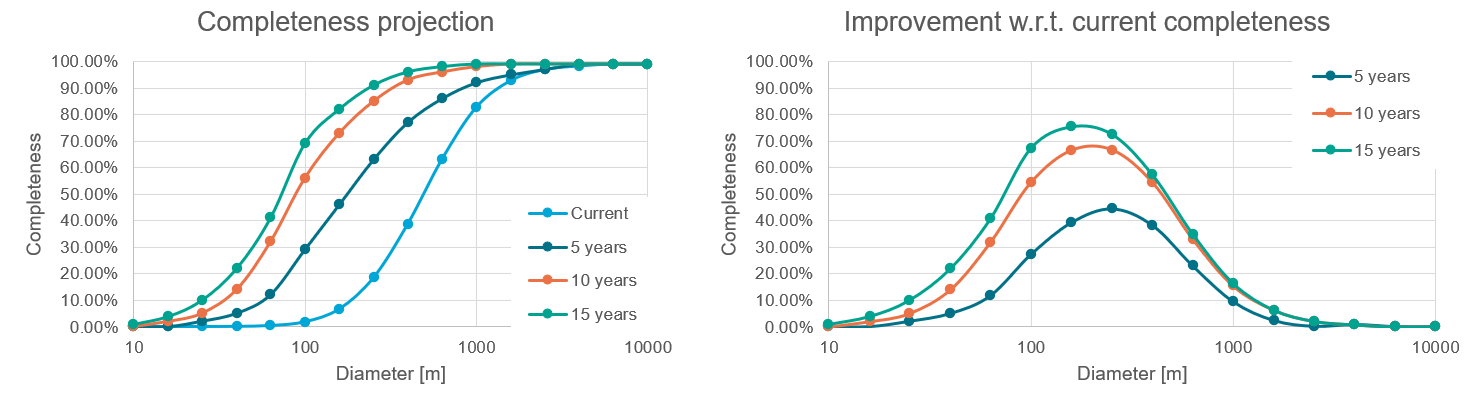
\includegraphics[width=1.0\textwidth]{img/completeness_projection.png}
 \caption{Projected improvement in survey completeness for a 5, 10 and 15 year survey from deep space. Data from \cite{2017NEOSDT}.}
 \label{fig:completeness_projection}
\end{figure}

\autoref{fig:completeness_projection} shows a projection for the improvement in survey completeness as a function of NEA diameter for a hypothetical deep space survey. A few thing are of note: Firstly, it is clear that such a survey can offer a sizeable improvement in cataloguing efforts, additionally leading to completion of the spaceguard goal in several years. However, several of the aforementioned missions currently under development also have this potential. What is more interesting is that, due to the thermal infrared telescope, cooled in deep space and largely free from interference by planets, is likely to detect a large number of small NEAs, which was hinted at by the success of the NEOWISE mission. But, the main bulk of the improvement is found in the $100 \mathrm{m} < D < 1000 \mathrm{m}$ range. Lastly, the diminishing returns of running a mission for longer become clear: as the number of undetected NEAs which fall within the limiting magnitude of the detector decreases, the performance decreases with it. \\

A second proposal among deep space surveys is the work of \cite{ThesisOlga}. Her work investigates the problem of asteroid impact last warning from space. This addresses the weakness in systems such as ATLAS which was showcased by the Chelyabinsk impactor: If an asteroid approaches Earth from the Sun, it is not possible to detect it in advance from Earth, as the glare of the Sun will overpower the signal of the asteroid. \cite{ThesisOlga} shows that a system at the solar sail displaced Sun-Earth L1 point will provide good improvement to the effort of asteroid impact last warning strategies. However, as previously discussed, this would still leave insufficient time for e.g. a deflection mission (for the interested reader, \cite{DefendingEarth} gives a good overview of mitigation strategies). In addition, although the performance is vastly increased, performance in detecting asteroids coming from the direction of the Sun is still limited.

From the above, it is clear that current efforts are insufficient to reach the set goals for NEA cataloguing. In addition, although future surveys will reach this goal, they will only detect a small fraction of small NEAs, not cataloguing the largest population of near-Earth objects. In fact, even proposed surveys which avoid all interference from the atmosphere, the Earth and the Moon will not be capable of reaching this goal with a single spacecraft. Limitations are imposed by the location of the spacecraft, the required number of observations, and interference from Solar glare.

